\section{Obtained Results}

This section presents the compilation results, simulation behavior, and test scenarios executed on the dual-sensor temperature monitoring system. The results demonstrate that the implemented system correctly acquires temperature data from both analog and digital sensors, applies signal conditioning with hysteresis and debounce filtering, and presents the processed information through both the LCD display and structured STDIO reports.

\subsection{Build Process}

The project was compiled using PlatformIO for the Arduino Mega 2560 target platform. The build process includes compilation of all lab-specific source files, the three reusable libraries (AnalogTempSensor, DigitalTempSensor, ThresholdAlert), and three libraries reused from previous labs (LcdDisplay, Led, StdioSerial), along with the external dependencies (FreeRTOS, OneWire, DallasTemperature, LiquidCrystal\_I2C).

\begin{figure}[H]
\centering
\IfFileExists{resources/ObtainedResults/build_results.png}{%
    
\includegraphics[width=0.85\textwidth]{resources/ObtainedResults/build_results.png}%
}{%
    \fbox{\parbox{0.83\textwidth}{\centering\color{gray}\small
        [Screenshot pending --- run \texttt{pio run -e lab3\_1} and\\
        capture the terminal output showing \texttt{[SUCCESS]}\\
        Save to resources/ObtainedResults/build\_results.png]}}%
}
\caption{PlatformIO build output for Lab 3.1 environment}
\label{fig:build_results}
\end{figure}

The build completed successfully with the following resource utilization:
\begin{itemize}
    \item \textbf{Flash memory}: 26\,122 bytes (10.3\% of 253\,952 bytes available). The firmware size is dominated by the FreeRTOS kernel, the DallasTemperature and OneWire libraries, and the LiquidCrystal\_I2C library.
    \item \textbf{RAM}: 1\,969 bytes (24.0\% of 8\,192 bytes available). This includes the static globals, shared data structures, and the three task stacks (each pre-allocated by FreeRTOS). The ATmega2560's 8 KB of SRAM provides comfortable headroom for additional functionality.
\end{itemize}

The relatively modest resource consumption demonstrates that the modular architecture does not introduce significant overhead. The layered driver abstractions compile to efficient code because most methods are short and inline-friendly, and the C++ object model adds minimal runtime cost on AVR targets.

\subsection{Simulation Startup}

Upon starting the Wokwi simulation, the system executes the initialization sequence defined in \texttt{lab3\_1Setup()}: STDIO serial initialization, synchronization primitive creation, and task spawning. The serial terminal displays the startup banner confirming that all components initialized correctly.

\begin{figure}[H]
\centering
\IfFileExists{resources/ObtainedResults/simulation_start.png}{%
    
\includegraphics[width=0.85\textwidth]{resources/ObtainedResults/simulation_start.png}%
}{%
    \fbox{\parbox{0.83\textwidth}{\centering\color{gray}\small
        [Screenshot pending --- start Wokwi simulation and capture the\\
        serial terminal showing the startup banner and initial readings.\\
        Save to resources/ObtainedResults/simulation\_start.png]}}%
}
\caption{Simulation startup --- serial terminal showing initialization banner}
\label{fig:simulation_start}
\end{figure}

After startup, the green LED turns on immediately (indicating normal operation), while the red and yellow LEDs remain off (indicating no alert conditions). The LCD displays the initial temperature readings on Page 0, showing the analog and digital sensor values along with the ``OK'' status indicators.

\subsection{Test Scenarios}

\subsubsection{Test 1: Normal Operation}

In normal operation, both sensors report temperatures below the 30\textdegree C high threshold. The system displays stable readings, the green LED remains solidly on, and both alert indicators (red and yellow LEDs) remain off.

\begin{figure}[H]
\centering
\IfFileExists{resources/ObtainedResults/test_normal_operation.png}{%
    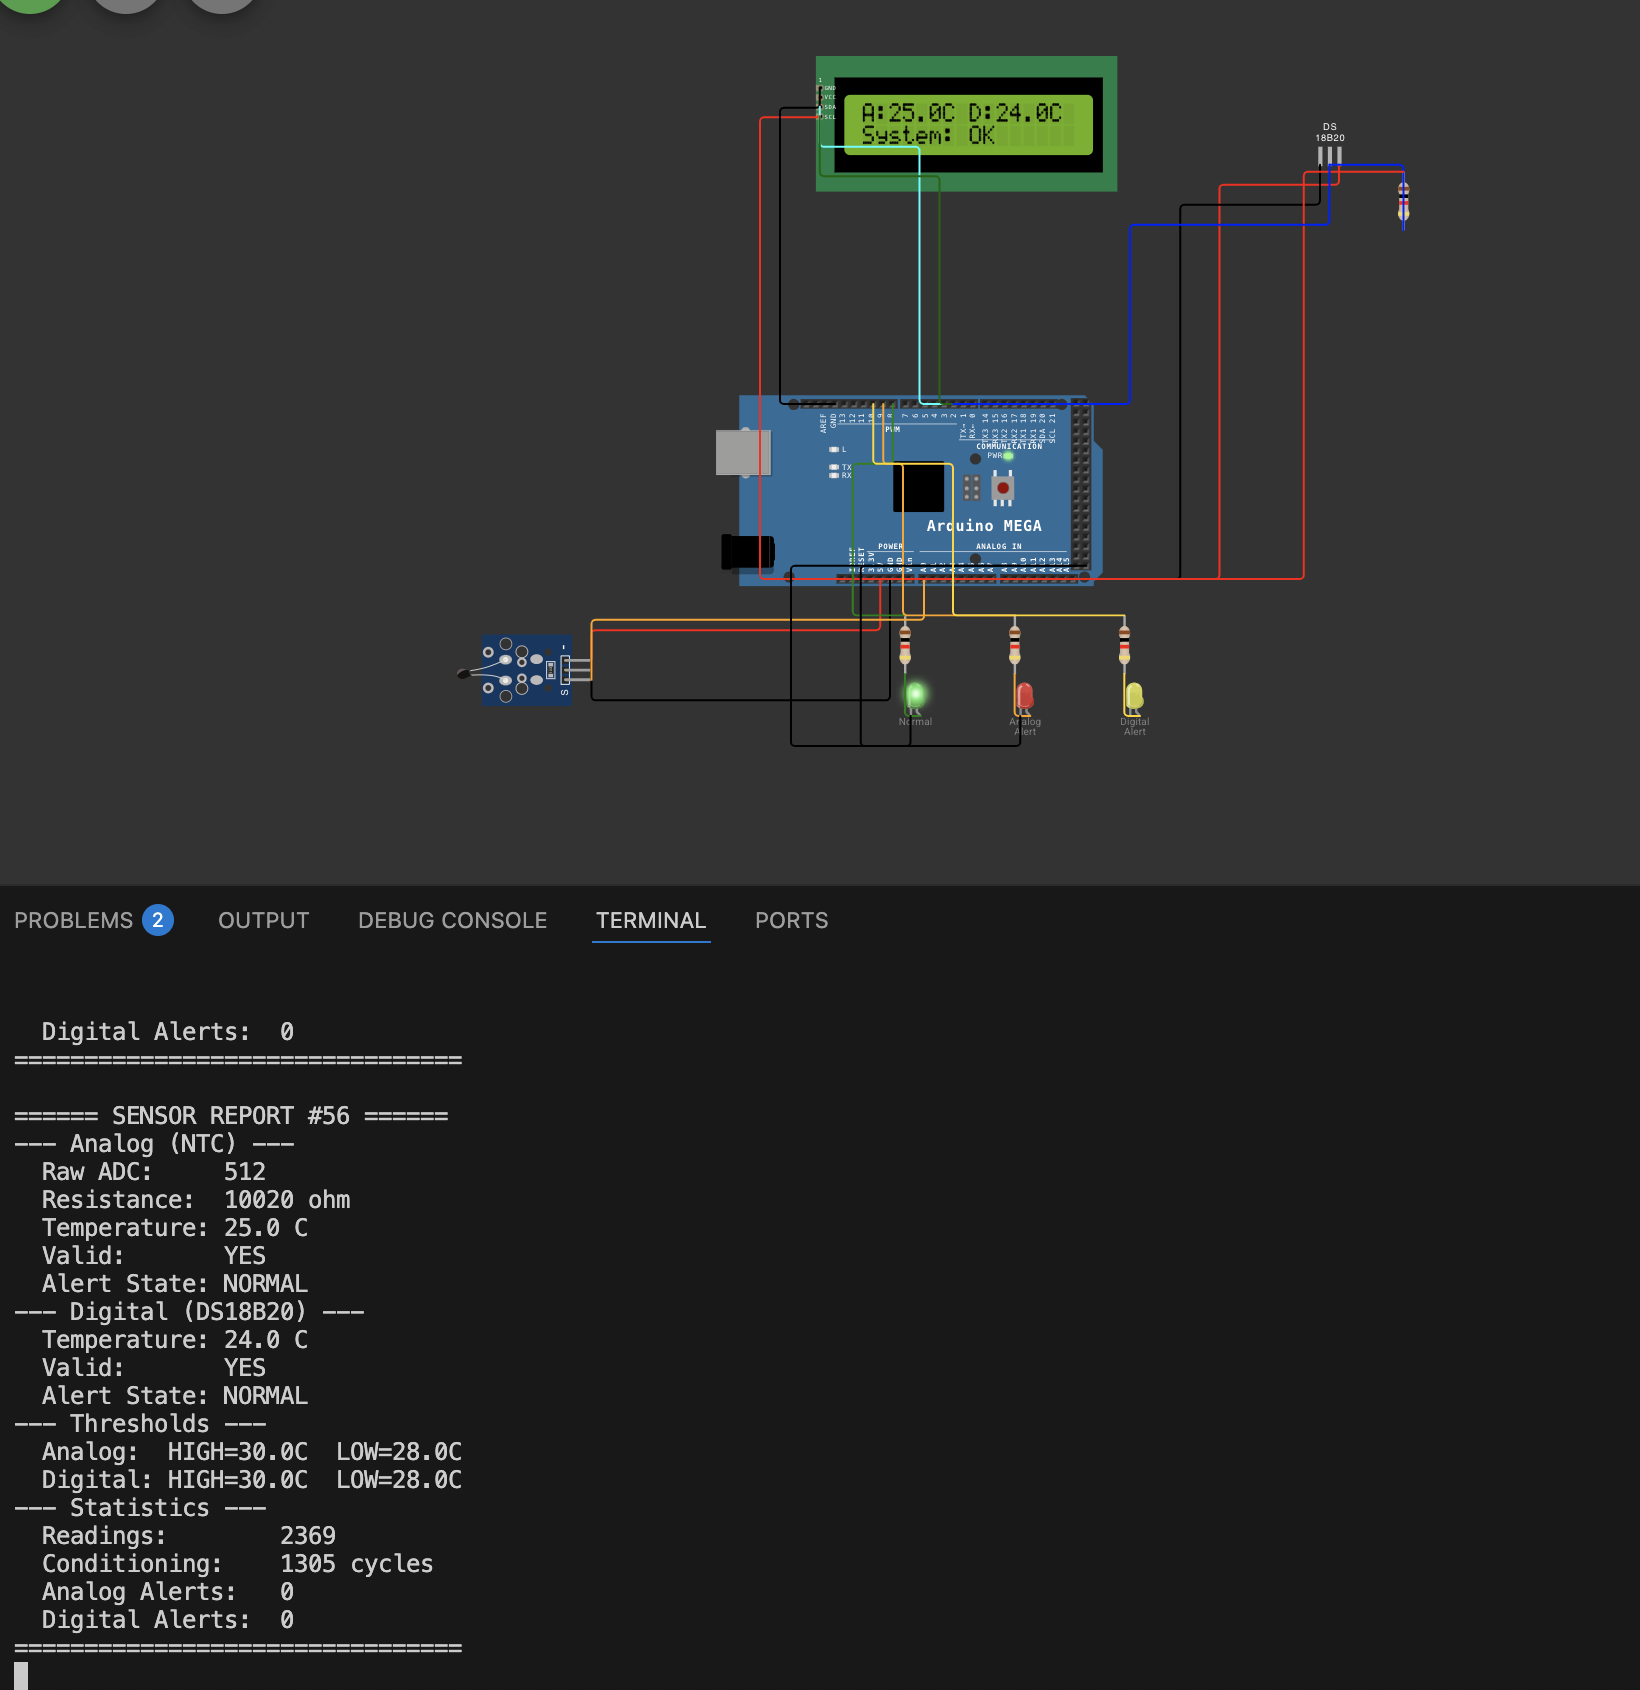
\includegraphics[width=0.85\textwidth]{resources/ObtainedResults/test_normal_operation.png}%
}{%
    \fbox{\parbox{0.83\textwidth}{\centering\color{gray}\small
        [Screenshot pending --- show Wokwi simulation with both sensors at\\
        room temperature (25\textdegree C). Green LED on, Red/Yellow LEDs off.\\
        LCD showing ``A:25.0C OK D:24.0C OK''.\\
        Save to resources/ObtainedResults/test\_normal\_operation.png]}}%
}
\caption{Normal operation --- both sensors below threshold}
\label{fig:test_normal}
\end{figure}

The STDIO report during normal operation shows all fields populated with valid data, alert states showing ``NORMAL'' for both sensors, and debounce counters at zero.

\subsubsection{Test 2: Analog Sensor Alert Trigger}

When the NTC thermistor temperature rises above 30\textdegree C (simulated by adjusting the NTC slider in Wokwi), the system transitions through the following sequence:
\begin{enumerate}
    \item The ThresholdAlert FSM for the analog channel moves from NORMAL to DEBOUNCE\_HIGH.
    \item The red LED begins blinking (toggling each conditioning cycle) during the debounce phase.
    \item After 5 consecutive readings above 30\textdegree C, the FSM transitions to ALERT\_ACTIVE.
    \item The red LED turns on solidly, and the green LED turns off.
    \item The LCD status changes from ``OK'' to ``!!'' for the analog channel.
\end{enumerate}

\begin{figure}[H]
\centering
\IfFileExists{resources/ObtainedResults/test_analog_alert.png}{%
    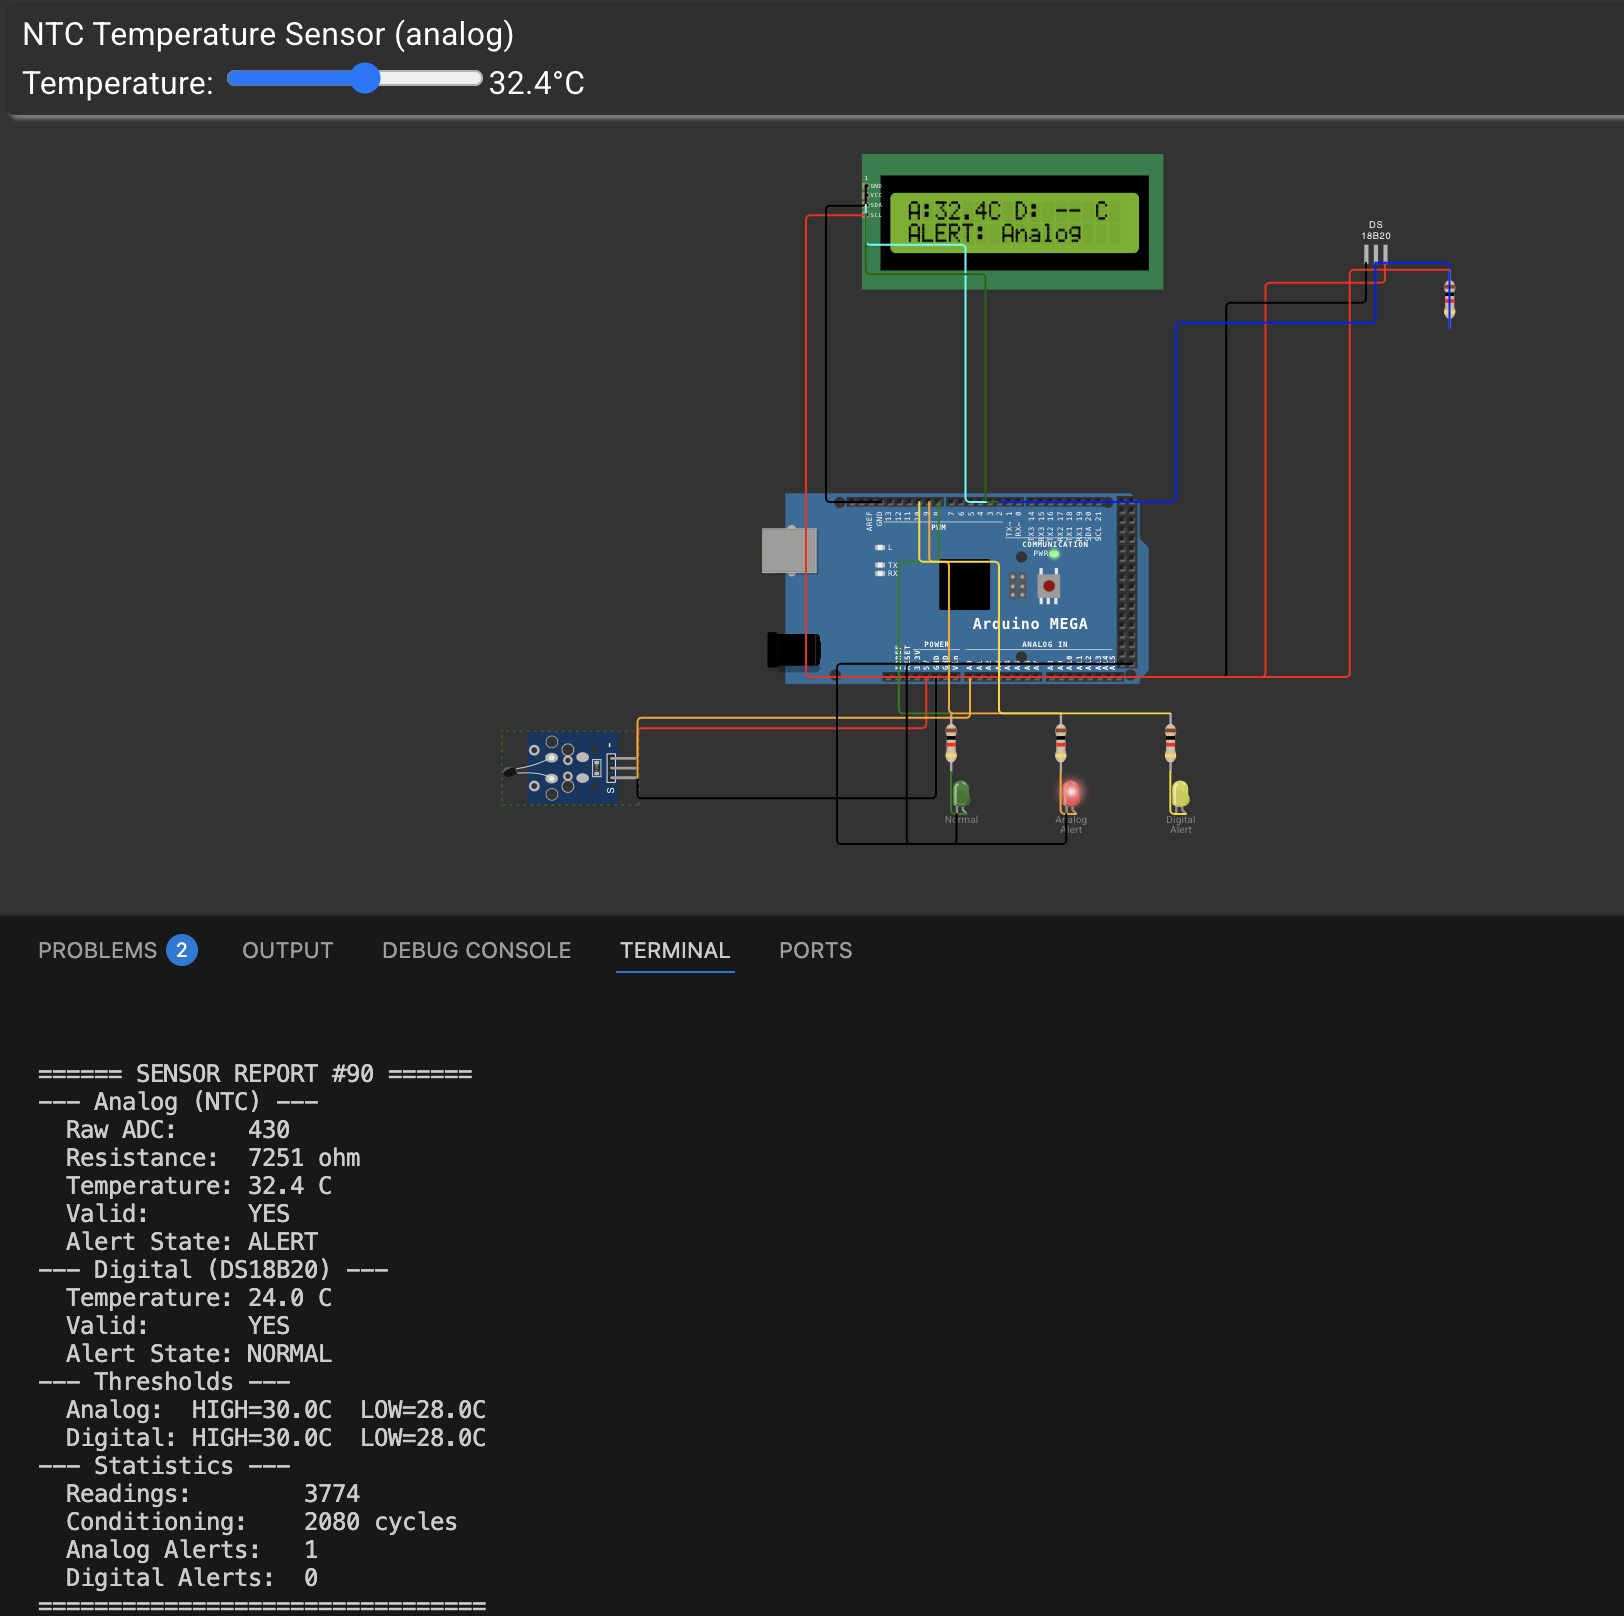
\includegraphics[width=0.85\textwidth]{resources/ObtainedResults/test_analog_alert.png}%
}{%
    \fbox{\parbox{0.83\textwidth}{\centering\color{gray}\small
        [Screenshot pending --- set NTC slider above 30\textdegree C in Wokwi.\\
        Red LED on, Green LED off, Yellow LED off.\\
        LCD showing ``A:32.5C !! D:24.0C OK''.\\
        Save to resources/ObtainedResults/test\_analog\_alert.png]}}%
}
\caption{Analog sensor alert --- NTC temperature above high threshold}
\label{fig:test_analog_alert}
\end{figure}

\subsubsection{Test 3: Digital Sensor Alert Trigger}

Similarly, when the DS18B20 temperature rises above 30\textdegree C (adjusted via the Wokwi temperature slider), the digital channel's ThresholdAlert FSM triggers independently. The yellow LED activates to indicate the digital alert, while the red LED state depends only on the analog channel.

\begin{figure}[H]
\centering
\IfFileExists{resources/ObtainedResults/test_digital_alert.png}{%
    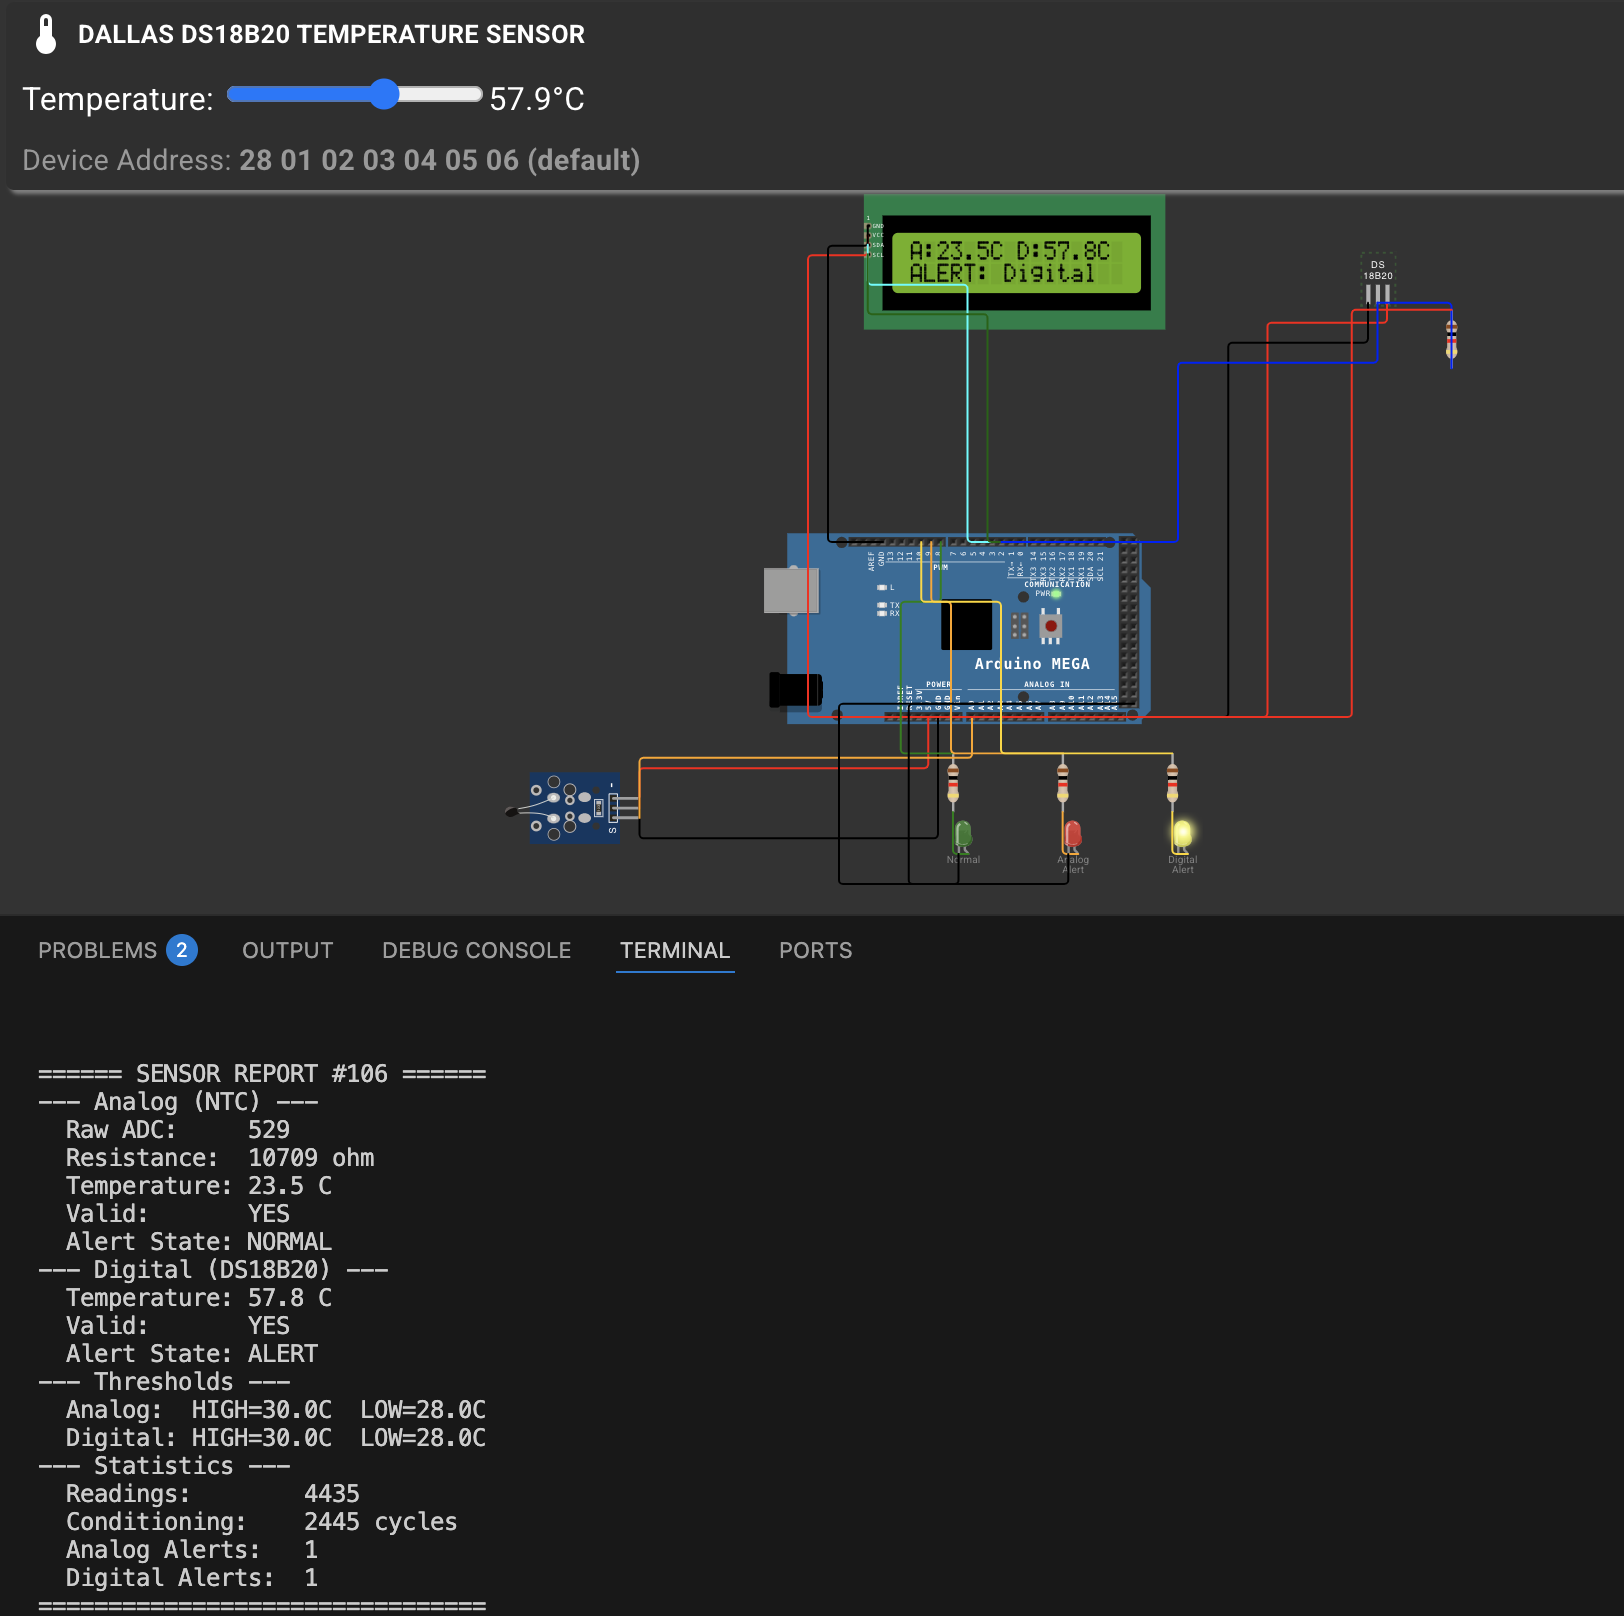
\includegraphics[width=0.85\textwidth]{resources/ObtainedResults/test_digital_alert.png}%
}{%
    \fbox{\parbox{0.83\textwidth}{\centering\color{gray}\small
        [Screenshot pending --- set DS18B20 slider above 30\textdegree C in Wokwi.\\
        Yellow LED on, Green LED off, Red LED off.\\
        LCD showing ``A:25.0C OK D:33.0C !!''.\\
        Save to resources/ObtainedResults/test\_digital\_alert.png]}}%
}
\caption{Digital sensor alert --- DS18B20 temperature above high threshold}
\label{fig:test_digital_alert}
\end{figure}

\subsubsection{Test 4: Dual Sensor Alert}

When both sensors simultaneously exceed the 30\textdegree C threshold, both the red and yellow LEDs activate, the green LED turns off, and the LCD shows ``!!'' status for both channels. This test verifies that the two ThresholdAlert instances operate independently and correctly.

\begin{figure}[H]
\centering
\IfFileExists{resources/ObtainedResults/test_dual_alert.png}{%
    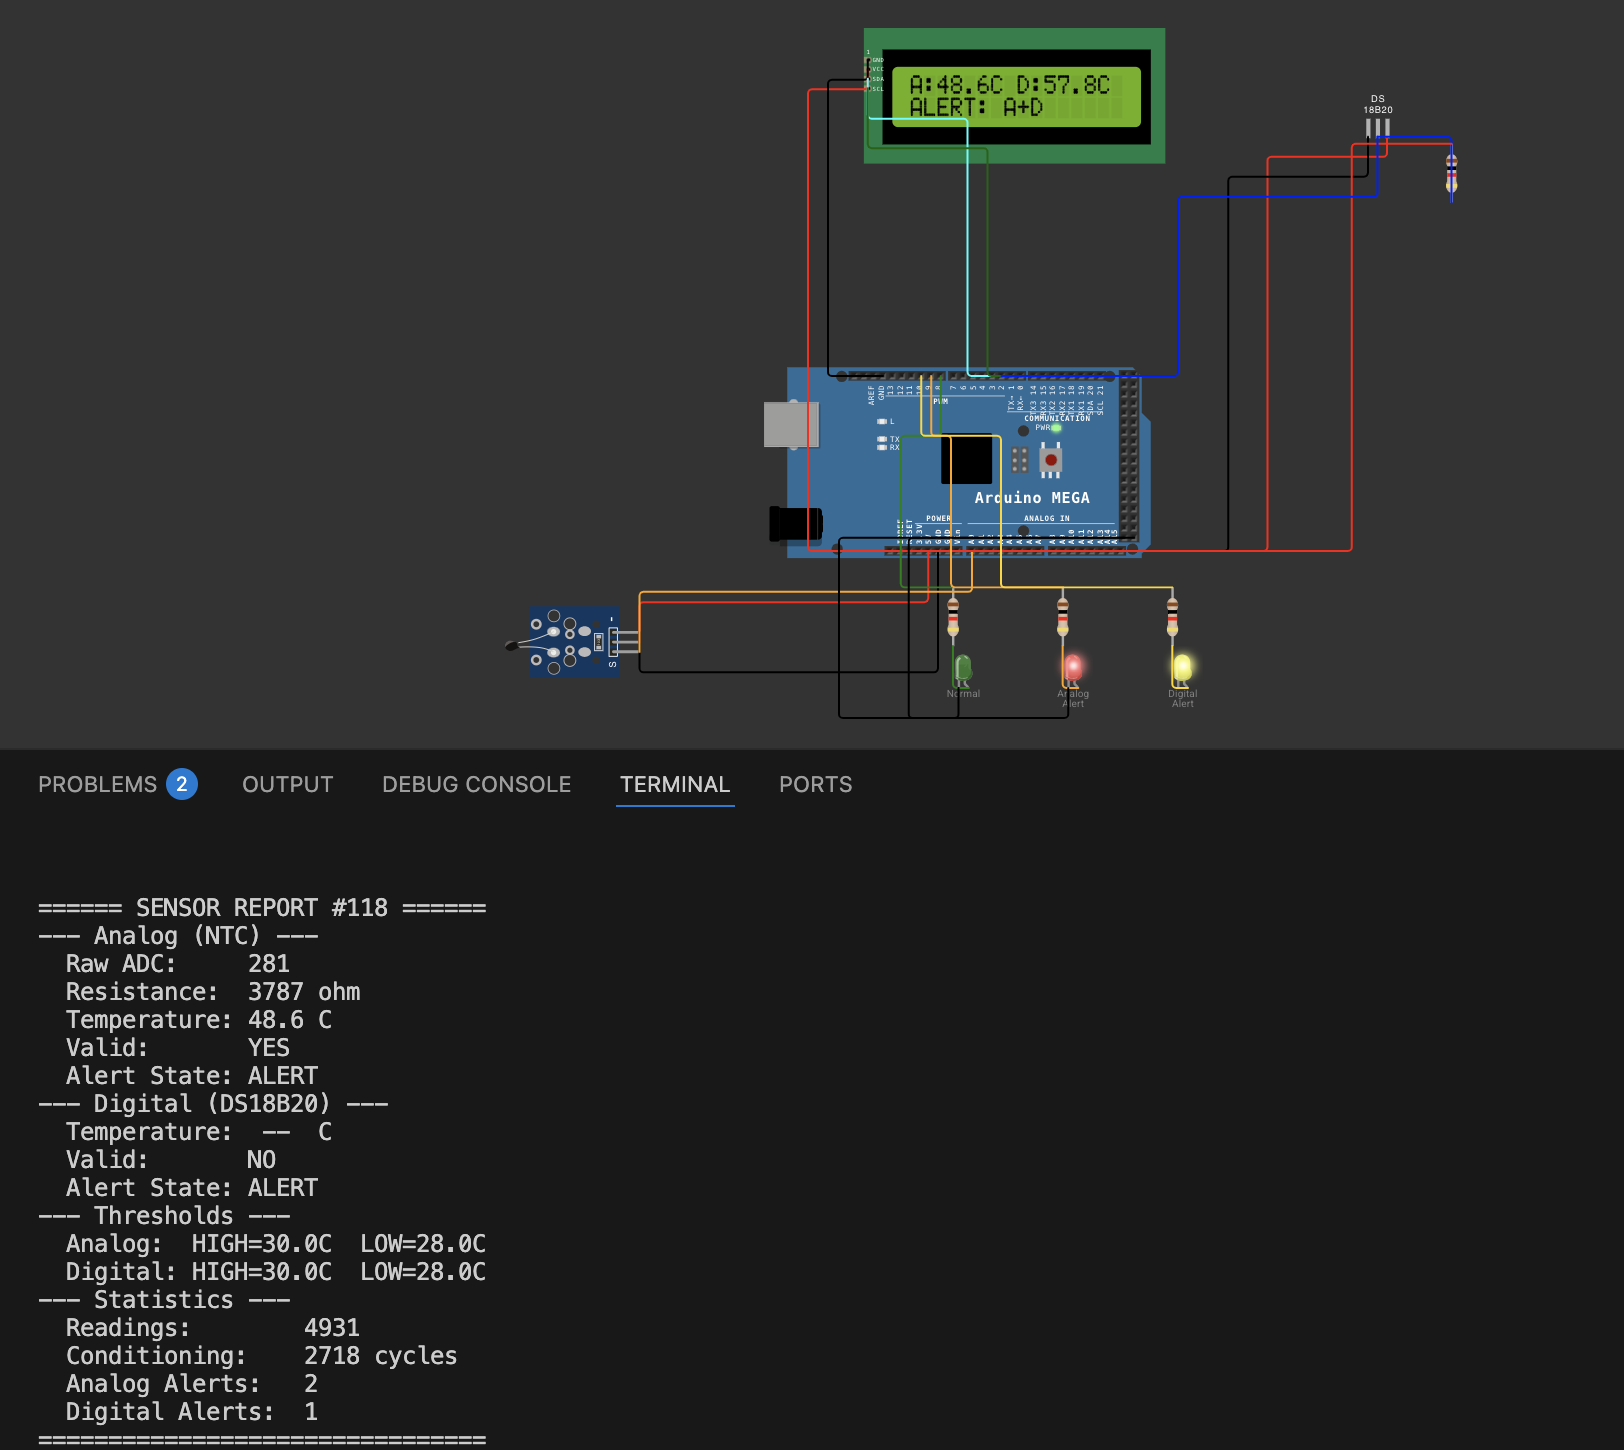
\includegraphics[width=0.85\textwidth]{resources/ObtainedResults/test_dual_alert.png}%
}{%
    \fbox{\parbox{0.83\textwidth}{\centering\color{gray}\small
        [Screenshot pending --- set both NTC and DS18B20 above 30\textdegree C.\\
        Red LED on, Yellow LED on, Green LED off.\\
        LCD showing ``A:32.5C !! D:33.0C !!''.\\
        Save to resources/ObtainedResults/test\_dual\_alert.png]}}%
}
\caption{Dual sensor alert --- both sensors above high threshold}
\label{fig:test_dual_alert}
\end{figure}

\subsubsection{Test 5: Hysteresis Behavior}

The hysteresis test demonstrates the dead-band between the high threshold (30\textdegree C) and the low threshold (28\textdegree C). Once an alert is active, the temperature must drop below 28\textdegree C (not just below 30\textdegree C) for the alert to clear. This prevents rapid toggling when the temperature oscillates near a single threshold value.

The test procedure is as follows:
\begin{enumerate}
    \item Start with the NTC temperature at 25\textdegree C (NORMAL state).
    \item Increase the temperature to 31\textdegree C $\rightarrow$ alert activates after debounce.
    \item Decrease to 29\textdegree C $\rightarrow$ alert remains active (above $T_{low}$ = 28\textdegree C).
    \item Decrease to 27\textdegree C $\rightarrow$ alert clears after debounce.
\end{enumerate}

\begin{figure}[H]
\centering
\IfFileExists{resources/ObtainedResults/test_hysteresis.png}{%
    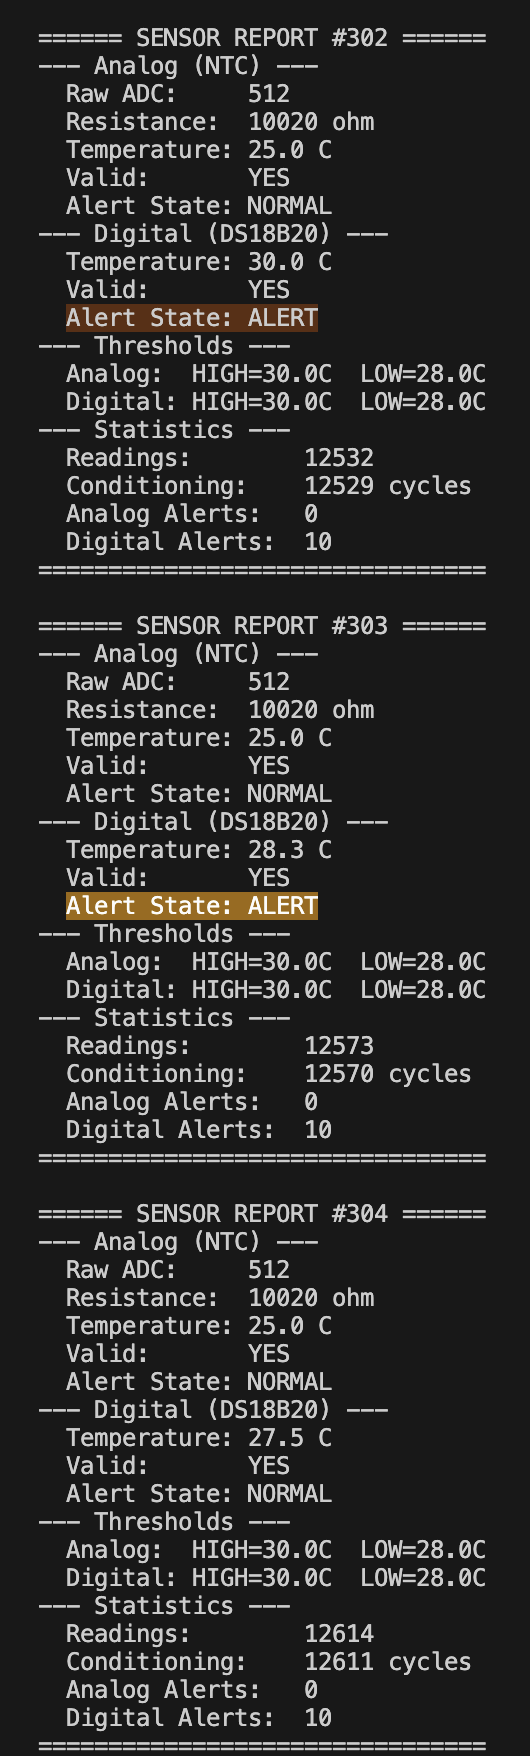
\includegraphics[width=0.85\textwidth]{resources/ObtainedResults/test_hysteresis.png}%
}{%
    \fbox{\parbox{0.83\textwidth}{\centering\color{gray}\small
        [Screenshot pending --- demonstrate hysteresis by lowering NTC\\
        from 31\textdegree C to 29\textdegree C (alert stays) then to 27\textdegree C (alert clears).\\
        Capture serial output showing state transitions.\\
        Save to resources/ObtainedResults/test\_hysteresis.png]}}%
}
\caption{Hysteresis behavior demonstration --- alert persists in dead-band zone}
\label{fig:test_hysteresis}
\end{figure}

\subsubsection{Test 6: Debounce Validation}

The debounce test validates that brief transient spikes do not trigger false alerts. By quickly adjusting the NTC temperature above and below 30\textdegree C (before 5 consecutive readings are accumulated), the system should return to NORMAL without entering ALERT\_ACTIVE.

\begin{figure}[H]
\centering
\IfFileExists{resources/ObtainedResults/test_debounce.png}{%
    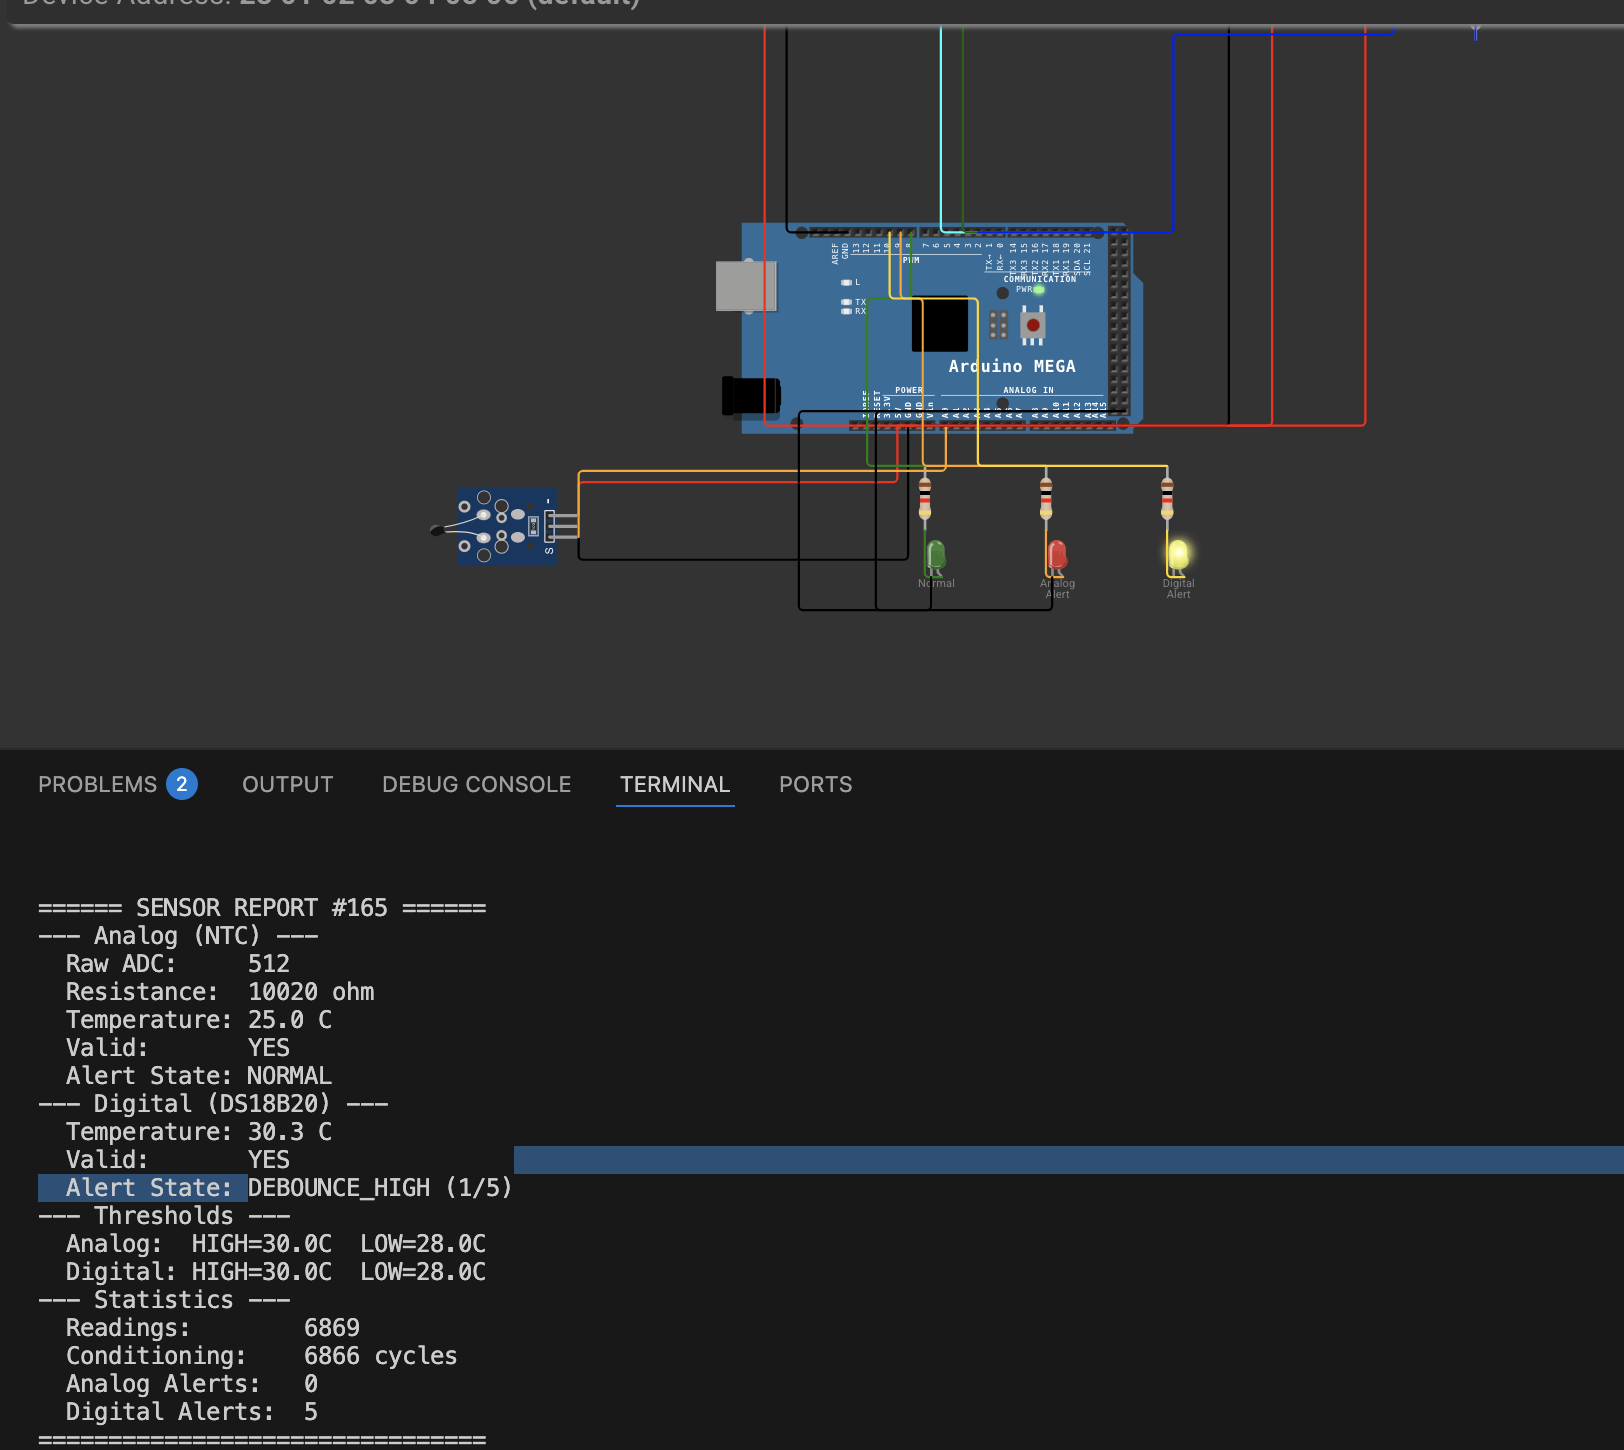
\includegraphics[width=0.85\textwidth]{resources/ObtainedResults/test_debounce.png}%
}{%
    \fbox{\parbox{0.83\textwidth}{\centering\color{gray}\small
        [Screenshot pending --- briefly raise NTC above 30\textdegree C then\\
        lower before 5 confirmations. Serial shows DB\_HIGH $\rightarrow$ NORMAL.\\
        Save to resources/ObtainedResults/test\_debounce.png]}}%
}
\caption{Debounce validation --- brief spike rejected by debounce filter}
\label{fig:test_debounce}
\end{figure}

\subsection{Serial Monitor Output}

The structured STDIO report generated every 2 seconds provides comprehensive diagnostic information. A typical report output includes raw ADC values, computed resistance, both temperatures, alert FSM states, debounce counters, cumulative statistics, and system uptime.

\begin{figure}[H]
\centering
\IfFileExists{resources/ObtainedResults/test_report.png}{%
    
\includegraphics[width=0.85\textwidth]{resources/ObtainedResults/test_report.png}%
}{%
    \fbox{\parbox{0.83\textwidth}{\centering\color{gray}\small
        [Screenshot pending --- capture the serial monitor showing\\
        a full structured STDIO report with all fields visible.\\
        Save to resources/ObtainedResults/test\_report.png]}}%
}
\caption{Structured STDIO diagnostic report from serial monitor}
\label{fig:test_report}
\end{figure}

The report includes the following fields:
\begin{itemize}
    \item \textbf{Sensor Readings}: Raw ADC value (0--1023), computed NTC resistance ($\Omega$), analog temperature (\textdegree C), digital temperature (\textdegree C), and validity flags.
    \item \textbf{Alert Status}: Current FSM state (NORMAL, DB\_HIGH, ALERT, DB\_LOW), debounce counter progress (e.g., ``3/5''), and filtered temperature value for both channels.
    \item \textbf{Statistics}: Total readings count, analog and digital alert activation counts, conditioning cycles, and system uptime in seconds.
\end{itemize}

\subsection{LCD Display Pages}

The LCD display alternates between two information pages every 500 ms:

\begin{itemize}
    \item \textbf{Page 0} shows the current temperature readings and alert status:
    \begin{verbatim}
    A:25.3C OK
    D:24.8C OK
    \end{verbatim}
    When an alert is active, the status changes from ``OK'' to ``!!''.

    \item \textbf{Page 1} shows the threshold configuration:
    \begin{verbatim}
    TH:30.0/28.0C
    Alerts: A:0 D:0
    \end{verbatim}
    The first line displays the high and low thresholds, and the second line shows the cumulative alert count for each channel.
\end{itemize}

\subsection{Verification Summary}

The following table summarizes the test results for all scenarios:

\begin{table}[H]
\centering
\begin{tabular}{|l|c|l|}
\hline
\textbf{Test Scenario} & \textbf{Result} & \textbf{Observation} \\
\hline
Normal operation         & PASS & Green LED on, no alerts \\
Analog alert trigger     & PASS & Red LED on after debounce \\
Digital alert trigger    & PASS & Yellow LED on after debounce \\
Dual sensor alert        & PASS & Both alert LEDs active \\
Hysteresis behavior      & PASS & Alert persists in dead-band \\
Debounce (false spike)   & PASS & Transient rejected \\
LCD page alternation     & PASS & Both pages display correctly \\
STDIO report format      & PASS & All fields populated \\
\hline
\end{tabular}
\caption{Test verification summary for Lab 3.1}
\label{tab:test_summary}
\end{table}

All test scenarios produced the expected behavior, confirming that the dual-sensor monitoring system correctly implements the signal acquisition, conditioning, and display pipeline as designed.
